\section{\label{sec:kbpo:kbpo} Implementing on-demand evaluation as an online service}

With all the components of the on-demand evaluation paradigm in place, we instantiated the paradigm on knowledge base population as a publicly available evaluation service dubbed KBP Online\footnote{Accessible at \url{https://kbpo.stanford.edu}}.
In this section, we'll outline the many practical considerations that were required to do so.

\subsection{Identifying the right query distributions}
As eluded to earlier, an extremely important design decision for our evaluation is determining \textit{which} set of entities and relations to query.
We looked to the evaluation guidelines of the TAC KBP competition developed by the Linguistic Development Consortium (LDC)~\citep{ellis2015tackbp,mayfield2012evaluating} as a well-respected community standard and tried to adapt it to our framework.

\begin{figure}
  \centering
  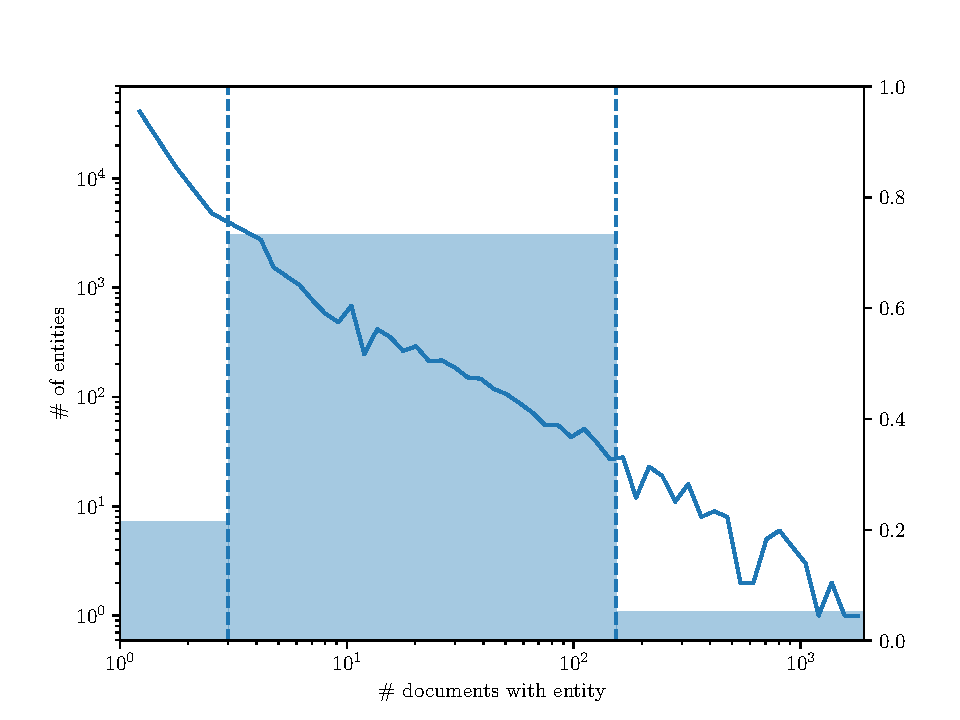
\includegraphics[width=0.8\textwidth]{figures/analysis/distribution}
  \caption[TAC KBP 2016 Query entity distribution]{\label{fig:kbpo:distribution}
    The solid line plots a histogram of how many documents a particular entity appeared in the TAC KBP 2016 corpus.
    The distribution is approximately a power-law distribution.
    Overlayed is a histogram of the frequency of the actual query entities used in the TAC KBP 2016 evaluation, binned by their frequency. We consider entities that appear in 3 or less unique documents (the 50th percentile) to be ``low'' frequency entities, those that appear more than 154 unique document (90th percentile) to be ``high'' frequency entities and those that appear in between to be ``medium'' frequency entities.
    The TAC KBP 2016 evaluation has a clear preference for medium frequency followed by low frequency entities.
  }
\end{figure}

\paragraph{The LDC query distribution and metrics.}
The first aspect we looked into was the distribution of entities that were queried in the official evaluations. 
The KBP evaluation is well known for using query entities that may have many relations but are still not common enough to have a knowledge base entry on say Wikipedia.
We wanted to capture this property in our evaluation as well.

To get a better sense of the distribution of entities that were queried, we used the entities (i.e., people and organizations) that were recognized by the Stanford KBP entity linking system~\citet{stanford2017kbp} and plotted a log-log distribution of the number of entities that appear in some number of documents (\reffig{kbpo:distribution}).
As one might expect, the distribution is extremely long-tailed: there are many entities that appear in just one or two documents. 
The distribution roughly follows a power-law distribution.

We then binned entities into three categories, ``low'' frequency entities that appear in at most 3 documents in the corpus (this is the 50th percentile), ``medium'' frequency entities that appear in between 3 and 154 (90th percentile) documents and finally, ``high'' frequency entities that appear in more than 154 documents.
The proportion of query entities in these three bins has been overlayed on top of the distribution in \reffig{kbpo:distribution}.
We see that a majority of the entities queried are medium frequency, followed by low frequency entities and a handful of high frequency entities.
We would like to ensure that our sampling distributions adequately capture these medium frequency entities. 

\begin{figure}
  \centering
  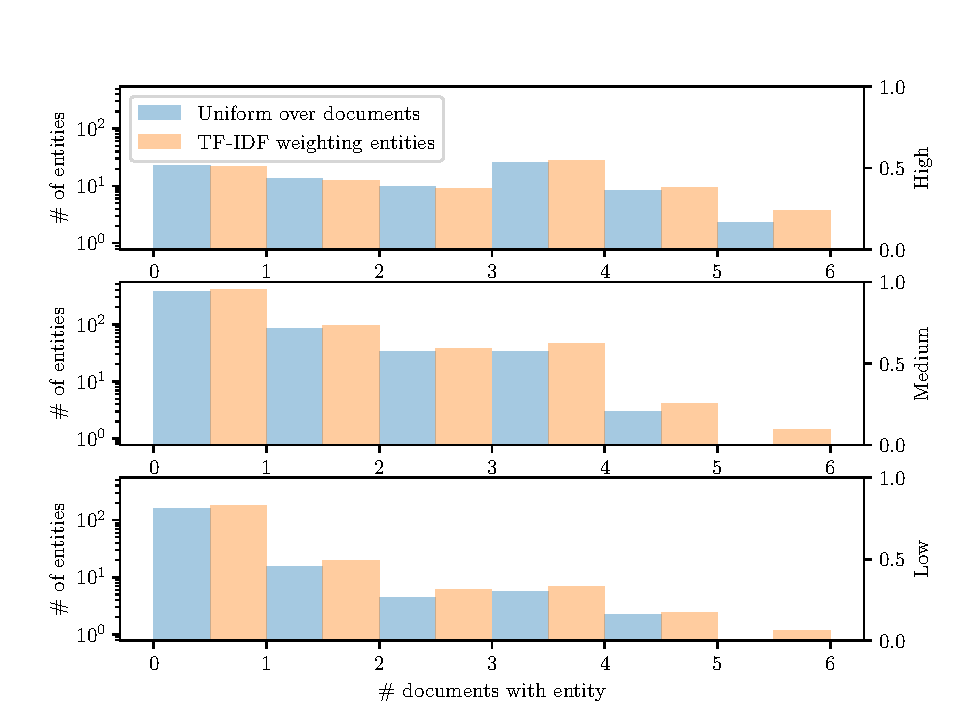
\includegraphics[width=0.8\textwidth]{figures/analysis/exhaustive_entity_cross}
  \caption[Comparison of document sampling distributions]{\label{fig:kbpo:exhaustive-entity}
  In order to properly test the entity linker when measuring recall, an important feature of KBP systems, we must identify documents for exhaustive annotation that contain some entity clusters.
  A sample of 200 documents uniformly picked from the document collection only exhibits clusters for high frequency entities.
  Our TF-IDF sampling scheme is able to ensure that even medium and low frequency entities appear across multiple documents in the sample.
  }
\end{figure}


\paragraph{Identifying diverse clustered documents.}
Next, we wanted to come up with a good distribution with which to query documents to exhaustively annotate.
It is not enough for us to ensure the documents contain a good distribution of medium frequency entities: we must also ensure that these entities appear in multiple documents to fairly test systems' entity linking components.

First, we tried using documents that were sampled uniformly from the corpus.
As \reffig{kbpo:exhaustive-entity} shows, 
a randomly sampled document contains a good range of low, medium and high frequency entities, but almost none of these entities are shared across the documents of the collection.
We note that the fact that low frequency entities dominate the entity distribution is to be expected because they constitute the majority of entities in any given document.\footnote{%
  We also tried sampling documents based on the frequency of entities they contained (estimated using the Stanford entity linker), but found that it did not significantly reduce the number of low frequency entities.}
We correct for this factor when sampling relations.

Instead, we used a two-step sampling procedure.
First, we would randomly sample documents for 20\% of our exhaustive document collection and then sample the remaining documents proportional to their aggregate TF-IDF scores with the entities identified in the first sample.
\reffig{exhaustive-entity} shows the distribution of entities that were sampled by this method, using the Stanford entity linking system to identify entities in the first sample.
When implementing this method in practice, we explicitly avoided using the Stanford entity linking system when identifying entities in documents because we were concerned about the bias it would introduce into our recall estimates.
Instead, we identified the entities in the first sample using crowdsourcing with our exhaustive annotation interface.

\begin{figure}
  \centering
  \begin{subfigure}{0.8\textwidth}
    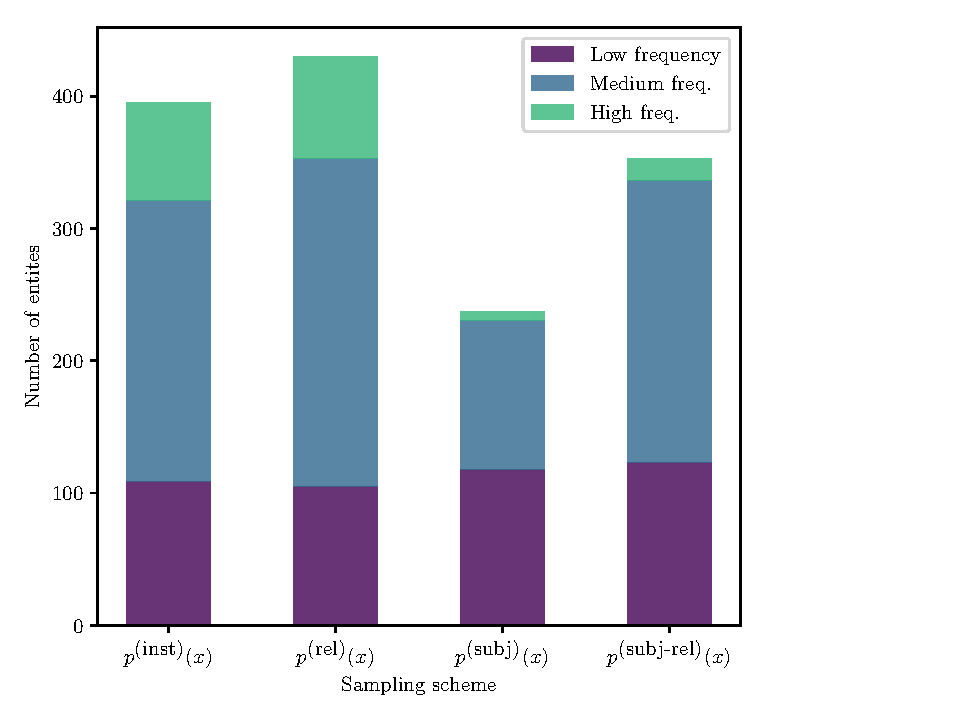
\includegraphics[width=\textwidth]{figures/analysis/selective_supervised_entity}
    \caption{Entity distribution}
  \end{subfigure}

  \begin{subfigure}{0.8\textwidth}
    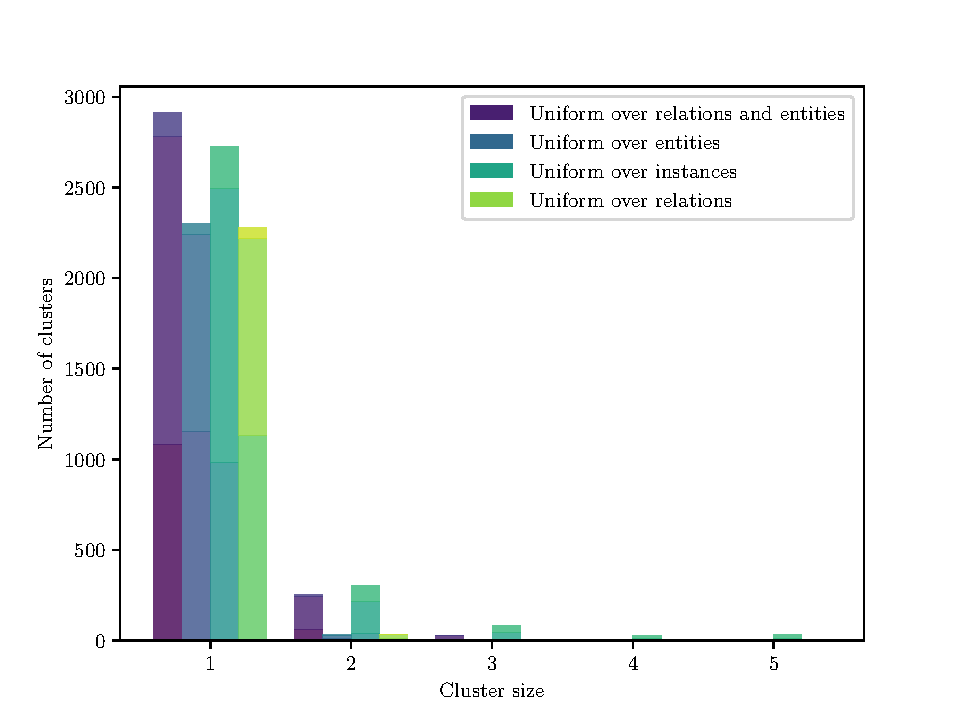
\includegraphics[width=\textwidth]{figures/analysis/selective_supervised_clusters}
    \caption{Entity cluster distribution}
  \end{subfigure}

  \caption[Comparison of relation sampling distributions]{\label{fig:kbpo:selective-supervised-entity}
  }
\end{figure}

\begin{figure}
  \centering
  \begin{subfigure}{\textwidth}
    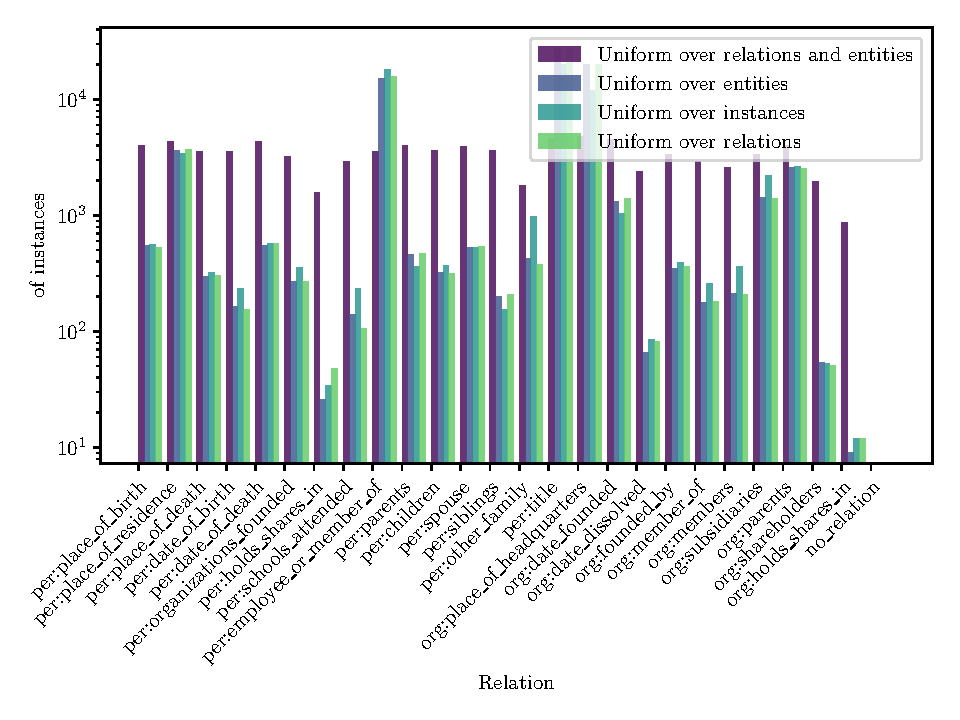
\includegraphics[width=\textwidth]{figures/analysis/selective_supervised_relations}
    \caption{Relation distribution}
  \end{subfigure}

  \caption[Comparison of relation sampling distributions]{\label{fig:kbpo:selective-supervised-relation}
  }
\end{figure}

\paragraph{Identifying diverse clustered relations.}
Finally, we wanted to ensure that the entities we sampled from systems were well distributed both over medium frequency entities and over relations.
Unsurprisingly, the naive approach of uniformly sampling relations outputted by systems, is dominated by a few common relations (e.g., \texttt{per:title}) on high frequency entities (\reffig{selective-supervised-entity}).

Our first attempt at rectifying the problem was to use two distributions that sampled relations inversely proportional to the frequency of their subject entity and relation label respectively:
\begin{align*}
  p^{\text{(subj)}}(x) &\propto \frac{1}{|\texttt{subj}(x)|} &
  p^{\text{(rel)}}(x) &\propto \frac{1}{|\texttt{rel}(x)|}
\end{align*}
These distributions solved these problems individually, but the samples collected on one did not transfer well to the other, reducing the effectiveness of reusing these samples.
There was an additional problem: we hardly ever selected two relations from the same entity, as shown in \reffig{selective-supervised-clusters}.
We wanted to maintain this property to be able to test the entity linking component of systems.

Our final proposed distribution rectified this by combining $p^{\text{(subj)}}(x)$ and $p^{\text{(rel)}}(x)$ and including a factor for the number of \textit{other} relations the subject label had.
\begin{align*}
  p^{\text{(subj-rel)}}(x) &\propto \frac{|\texttt{subj-relns}(x)|}{|\texttt{subj}(x)| |\texttt{rel}(x)|},
\end{align*}
\reffig{selective-supervised-entity} shows how this new distribution has both a better representation of medium frequency entities and is well balanced across all the relations.
\reffig{selective-supervised-clusters} also shows that it is able to represent some entities with multiple relations. 

\begin{figure}
  \centering
  \begin{subfigure}{0.8\textwidth}
    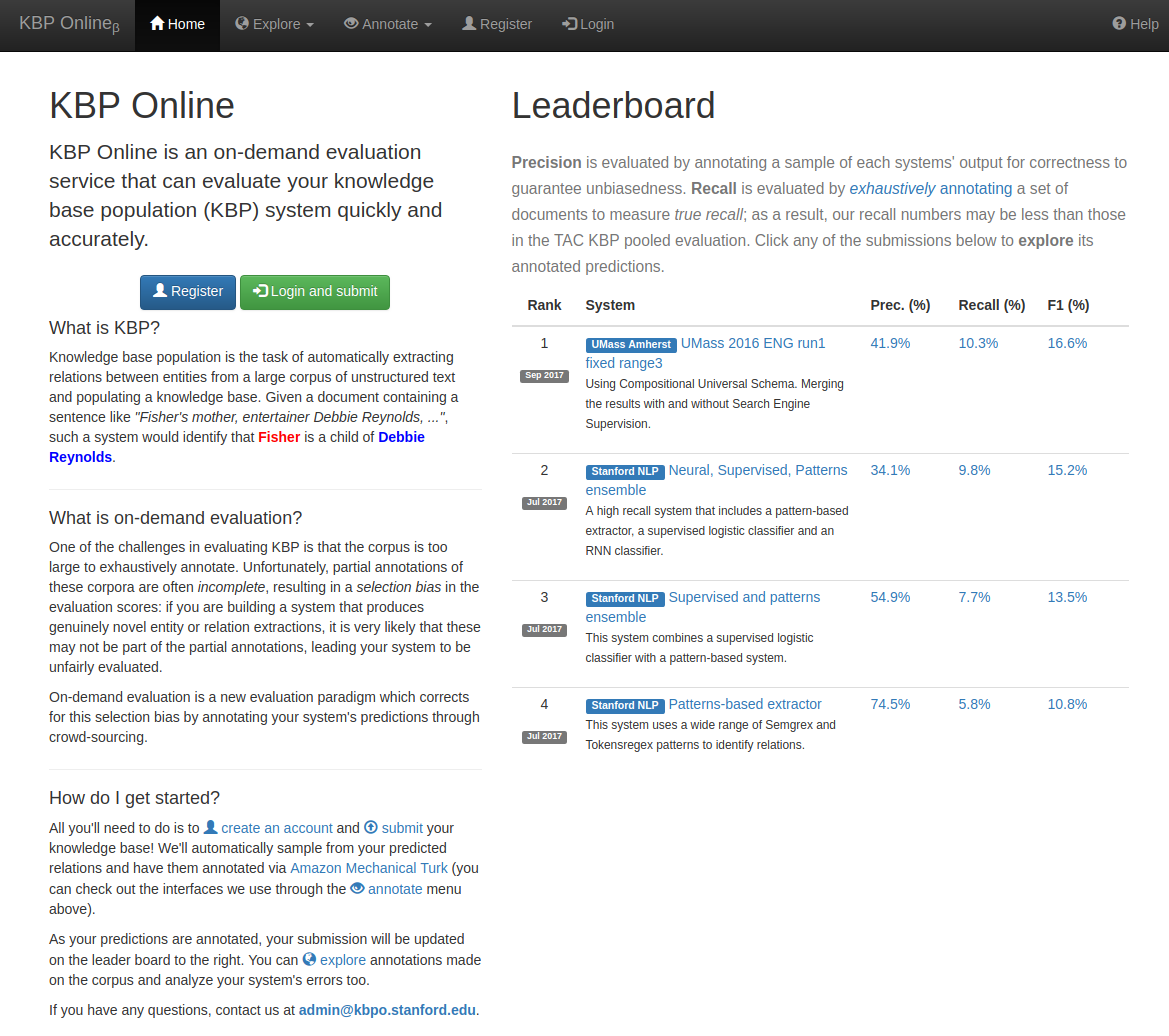
\includegraphics[width=\textwidth]{figures/interface/leaderboard}
    \caption{Leaderboard}
  \end{subfigure}

  \begin{subfigure}{0.8\textwidth}
    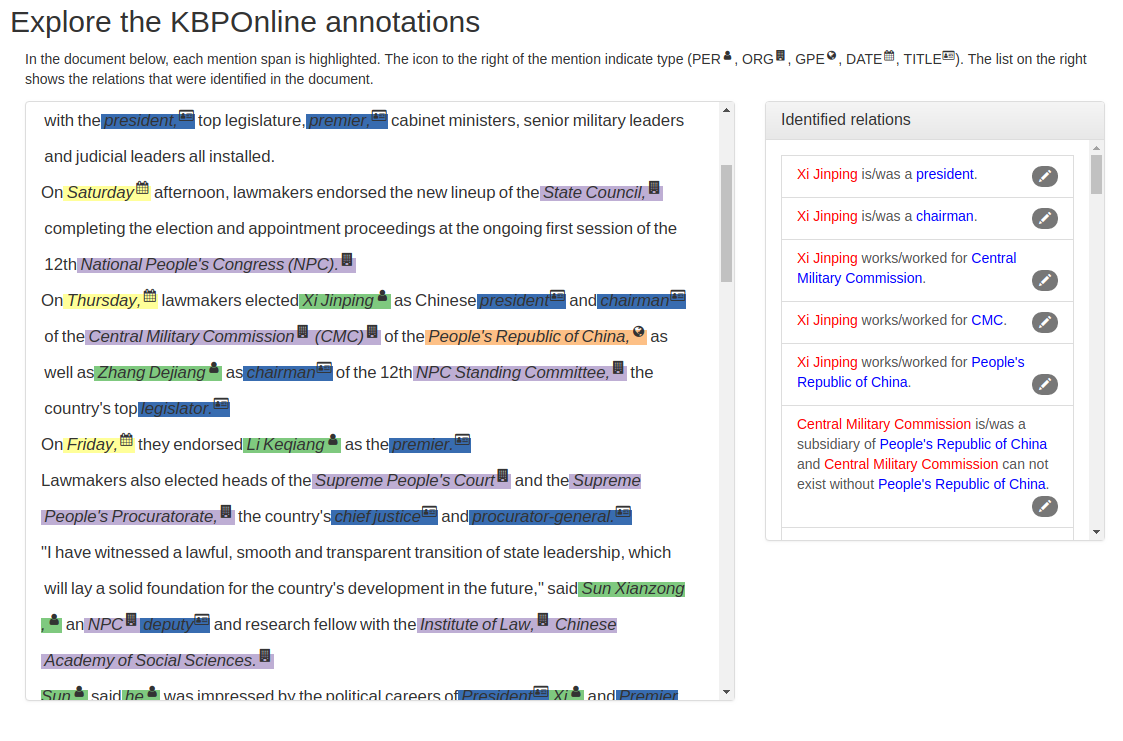
\includegraphics[width=\textwidth]{figures/interface/explore-data}
    \caption{Explore annotations}
  \end{subfigure}

  \begin{subfigure}{0.8\textwidth}
    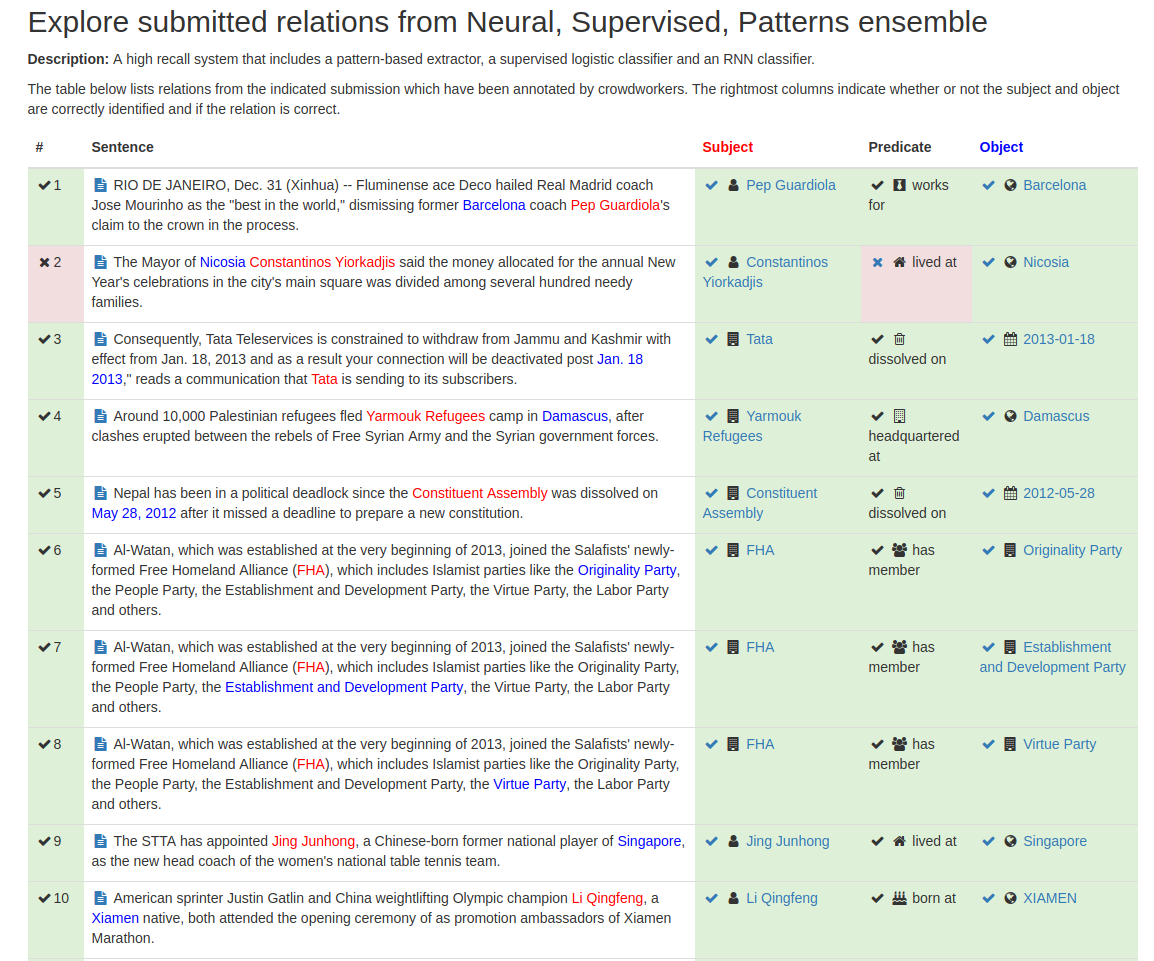
\includegraphics[width=\textwidth]{figures/interface/errors}
    \caption{Error analysis}
  \end{subfigure}

  \caption[KBP Online]{\label{fig:kbpo:kbpo}
  }
\end{figure}

\section{Implementation details}
Implemented with postgres, django, remote calls to Amazon Mechanical Turk.
Parse input using official format.
We integrated the crowdsourcing interfaces described in \refsec{application} to dynamically launch crowdsourcing tasks as 
asynchronous turking requests

\subsection{Computing scores}
Handle entity linking.

\subsection{Error analysis}
Use the distributions to do accurately break down by relations.

